% Options for packages loaded elsewhere
\PassOptionsToPackage{unicode}{hyperref}
\PassOptionsToPackage{hyphens}{url}
\PassOptionsToPackage{dvipsnames,svgnames,x11names}{xcolor}
%
\documentclass[
  letterpaper,
  DIV=11,
  numbers=noendperiod]{scrreprt}

\usepackage{amsmath,amssymb}
\usepackage{lmodern}
\usepackage{iftex}
\ifPDFTeX
  \usepackage[T1]{fontenc}
  \usepackage[utf8]{inputenc}
  \usepackage{textcomp} % provide euro and other symbols
\else % if luatex or xetex
  \usepackage{unicode-math}
  \defaultfontfeatures{Scale=MatchLowercase}
  \defaultfontfeatures[\rmfamily]{Ligatures=TeX,Scale=1}
\fi
% Use upquote if available, for straight quotes in verbatim environments
\IfFileExists{upquote.sty}{\usepackage{upquote}}{}
\IfFileExists{microtype.sty}{% use microtype if available
  \usepackage[]{microtype}
  \UseMicrotypeSet[protrusion]{basicmath} % disable protrusion for tt fonts
}{}
\makeatletter
\@ifundefined{KOMAClassName}{% if non-KOMA class
  \IfFileExists{parskip.sty}{%
    \usepackage{parskip}
  }{% else
    \setlength{\parindent}{0pt}
    \setlength{\parskip}{6pt plus 2pt minus 1pt}}
}{% if KOMA class
  \KOMAoptions{parskip=half}}
\makeatother
\usepackage{xcolor}
\setlength{\emergencystretch}{3em} % prevent overfull lines
\setcounter{secnumdepth}{5}
% Make \paragraph and \subparagraph free-standing
\ifx\paragraph\undefined\else
  \let\oldparagraph\paragraph
  \renewcommand{\paragraph}[1]{\oldparagraph{#1}\mbox{}}
\fi
\ifx\subparagraph\undefined\else
  \let\oldsubparagraph\subparagraph
  \renewcommand{\subparagraph}[1]{\oldsubparagraph{#1}\mbox{}}
\fi

\usepackage{color}
\usepackage{fancyvrb}
\newcommand{\VerbBar}{|}
\newcommand{\VERB}{\Verb[commandchars=\\\{\}]}
\DefineVerbatimEnvironment{Highlighting}{Verbatim}{commandchars=\\\{\}}
% Add ',fontsize=\small' for more characters per line
\usepackage{framed}
\definecolor{shadecolor}{RGB}{241,243,245}
\newenvironment{Shaded}{\begin{snugshade}}{\end{snugshade}}
\newcommand{\AlertTok}[1]{\textcolor[rgb]{0.68,0.00,0.00}{#1}}
\newcommand{\AnnotationTok}[1]{\textcolor[rgb]{0.37,0.37,0.37}{#1}}
\newcommand{\AttributeTok}[1]{\textcolor[rgb]{0.40,0.45,0.13}{#1}}
\newcommand{\BaseNTok}[1]{\textcolor[rgb]{0.68,0.00,0.00}{#1}}
\newcommand{\BuiltInTok}[1]{\textcolor[rgb]{0.00,0.23,0.31}{#1}}
\newcommand{\CharTok}[1]{\textcolor[rgb]{0.13,0.47,0.30}{#1}}
\newcommand{\CommentTok}[1]{\textcolor[rgb]{0.37,0.37,0.37}{#1}}
\newcommand{\CommentVarTok}[1]{\textcolor[rgb]{0.37,0.37,0.37}{\textit{#1}}}
\newcommand{\ConstantTok}[1]{\textcolor[rgb]{0.56,0.35,0.01}{#1}}
\newcommand{\ControlFlowTok}[1]{\textcolor[rgb]{0.00,0.23,0.31}{#1}}
\newcommand{\DataTypeTok}[1]{\textcolor[rgb]{0.68,0.00,0.00}{#1}}
\newcommand{\DecValTok}[1]{\textcolor[rgb]{0.68,0.00,0.00}{#1}}
\newcommand{\DocumentationTok}[1]{\textcolor[rgb]{0.37,0.37,0.37}{\textit{#1}}}
\newcommand{\ErrorTok}[1]{\textcolor[rgb]{0.68,0.00,0.00}{#1}}
\newcommand{\ExtensionTok}[1]{\textcolor[rgb]{0.00,0.23,0.31}{#1}}
\newcommand{\FloatTok}[1]{\textcolor[rgb]{0.68,0.00,0.00}{#1}}
\newcommand{\FunctionTok}[1]{\textcolor[rgb]{0.28,0.35,0.67}{#1}}
\newcommand{\ImportTok}[1]{\textcolor[rgb]{0.00,0.46,0.62}{#1}}
\newcommand{\InformationTok}[1]{\textcolor[rgb]{0.37,0.37,0.37}{#1}}
\newcommand{\KeywordTok}[1]{\textcolor[rgb]{0.00,0.23,0.31}{#1}}
\newcommand{\NormalTok}[1]{\textcolor[rgb]{0.00,0.23,0.31}{#1}}
\newcommand{\OperatorTok}[1]{\textcolor[rgb]{0.37,0.37,0.37}{#1}}
\newcommand{\OtherTok}[1]{\textcolor[rgb]{0.00,0.23,0.31}{#1}}
\newcommand{\PreprocessorTok}[1]{\textcolor[rgb]{0.68,0.00,0.00}{#1}}
\newcommand{\RegionMarkerTok}[1]{\textcolor[rgb]{0.00,0.23,0.31}{#1}}
\newcommand{\SpecialCharTok}[1]{\textcolor[rgb]{0.37,0.37,0.37}{#1}}
\newcommand{\SpecialStringTok}[1]{\textcolor[rgb]{0.13,0.47,0.30}{#1}}
\newcommand{\StringTok}[1]{\textcolor[rgb]{0.13,0.47,0.30}{#1}}
\newcommand{\VariableTok}[1]{\textcolor[rgb]{0.07,0.07,0.07}{#1}}
\newcommand{\VerbatimStringTok}[1]{\textcolor[rgb]{0.13,0.47,0.30}{#1}}
\newcommand{\WarningTok}[1]{\textcolor[rgb]{0.37,0.37,0.37}{\textit{#1}}}

\providecommand{\tightlist}{%
  \setlength{\itemsep}{0pt}\setlength{\parskip}{0pt}}\usepackage{longtable,booktabs,array}
\usepackage{calc} % for calculating minipage widths
% Correct order of tables after \paragraph or \subparagraph
\usepackage{etoolbox}
\makeatletter
\patchcmd\longtable{\par}{\if@noskipsec\mbox{}\fi\par}{}{}
\makeatother
% Allow footnotes in longtable head/foot
\IfFileExists{footnotehyper.sty}{\usepackage{footnotehyper}}{\usepackage{footnote}}
\makesavenoteenv{longtable}
\usepackage{graphicx}
\makeatletter
\def\maxwidth{\ifdim\Gin@nat@width>\linewidth\linewidth\else\Gin@nat@width\fi}
\def\maxheight{\ifdim\Gin@nat@height>\textheight\textheight\else\Gin@nat@height\fi}
\makeatother
% Scale images if necessary, so that they will not overflow the page
% margins by default, and it is still possible to overwrite the defaults
% using explicit options in \includegraphics[width, height, ...]{}
\setkeys{Gin}{width=\maxwidth,height=\maxheight,keepaspectratio}
% Set default figure placement to htbp
\makeatletter
\def\fps@figure{htbp}
\makeatother
\newlength{\cslhangindent}
\setlength{\cslhangindent}{1.5em}
\newlength{\csllabelwidth}
\setlength{\csllabelwidth}{3em}
\newlength{\cslentryspacingunit} % times entry-spacing
\setlength{\cslentryspacingunit}{\parskip}
\newenvironment{CSLReferences}[2] % #1 hanging-ident, #2 entry spacing
 {% don't indent paragraphs
  \setlength{\parindent}{0pt}
  % turn on hanging indent if param 1 is 1
  \ifodd #1
  \let\oldpar\par
  \def\par{\hangindent=\cslhangindent\oldpar}
  \fi
  % set entry spacing
  \setlength{\parskip}{#2\cslentryspacingunit}
 }%
 {}
\usepackage{calc}
\newcommand{\CSLBlock}[1]{#1\hfill\break}
\newcommand{\CSLLeftMargin}[1]{\parbox[t]{\csllabelwidth}{#1}}
\newcommand{\CSLRightInline}[1]{\parbox[t]{\linewidth - \csllabelwidth}{#1}\break}
\newcommand{\CSLIndent}[1]{\hspace{\cslhangindent}#1}

\KOMAoption{captions}{tableheading}
\makeatletter
\@ifpackageloaded{tcolorbox}{}{\usepackage[many]{tcolorbox}}
\@ifpackageloaded{fontawesome5}{}{\usepackage{fontawesome5}}
\definecolor{quarto-callout-color}{HTML}{909090}
\definecolor{quarto-callout-note-color}{HTML}{0758E5}
\definecolor{quarto-callout-important-color}{HTML}{CC1914}
\definecolor{quarto-callout-warning-color}{HTML}{EB9113}
\definecolor{quarto-callout-tip-color}{HTML}{00A047}
\definecolor{quarto-callout-caution-color}{HTML}{FC5300}
\definecolor{quarto-callout-color-frame}{HTML}{acacac}
\definecolor{quarto-callout-note-color-frame}{HTML}{4582ec}
\definecolor{quarto-callout-important-color-frame}{HTML}{d9534f}
\definecolor{quarto-callout-warning-color-frame}{HTML}{f0ad4e}
\definecolor{quarto-callout-tip-color-frame}{HTML}{02b875}
\definecolor{quarto-callout-caution-color-frame}{HTML}{fd7e14}
\makeatother
\makeatletter
\makeatother
\makeatletter
\@ifpackageloaded{bookmark}{}{\usepackage{bookmark}}
\makeatother
\makeatletter
\@ifpackageloaded{caption}{}{\usepackage{caption}}
\AtBeginDocument{%
\ifdefined\contentsname
  \renewcommand*\contentsname{Table of contents}
\else
  \newcommand\contentsname{Table of contents}
\fi
\ifdefined\listfigurename
  \renewcommand*\listfigurename{List of Figures}
\else
  \newcommand\listfigurename{List of Figures}
\fi
\ifdefined\listtablename
  \renewcommand*\listtablename{List of Tables}
\else
  \newcommand\listtablename{List of Tables}
\fi
\ifdefined\figurename
  \renewcommand*\figurename{Figure}
\else
  \newcommand\figurename{Figure}
\fi
\ifdefined\tablename
  \renewcommand*\tablename{Table}
\else
  \newcommand\tablename{Table}
\fi
}
\@ifpackageloaded{float}{}{\usepackage{float}}
\floatstyle{ruled}
\@ifundefined{c@chapter}{\newfloat{codelisting}{h}{lop}}{\newfloat{codelisting}{h}{lop}[chapter]}
\floatname{codelisting}{Listing}
\newcommand*\listoflistings{\listof{codelisting}{List of Listings}}
\makeatother
\makeatletter
\@ifpackageloaded{caption}{}{\usepackage{caption}}
\@ifpackageloaded{subcaption}{}{\usepackage{subcaption}}
\makeatother
\makeatletter
\@ifpackageloaded{tcolorbox}{}{\usepackage[many]{tcolorbox}}
\makeatother
\makeatletter
\@ifundefined{shadecolor}{\definecolor{shadecolor}{rgb}{.97, .97, .97}}
\makeatother
\makeatletter
\makeatother
\ifLuaTeX
  \usepackage{selnolig}  % disable illegal ligatures
\fi
\IfFileExists{bookmark.sty}{\usepackage{bookmark}}{\usepackage{hyperref}}
\IfFileExists{xurl.sty}{\usepackage{xurl}}{} % add URL line breaks if available
\urlstyle{same} % disable monospaced font for URLs
\hypersetup{
  pdftitle={Data handling for biological sciences},
  colorlinks=true,
  linkcolor={blue},
  filecolor={Maroon},
  citecolor={Blue},
  urlcolor={Blue},
  pdfcreator={LaTeX via pandoc}}

\title{Data handling for biological sciences}
\usepackage{etoolbox}
\makeatletter
\providecommand{\subtitle}[1]{% add subtitle to \maketitle
  \apptocmd{\@title}{\par {\large #1 \par}}{}{}
}
\makeatother
\subtitle{Theoretical aspects and examples using R programming language}
\author{}
\date{}

\begin{document}
\maketitle
\ifdefined\Shaded\renewenvironment{Shaded}{\begin{tcolorbox}[breakable, boxrule=0pt, enhanced, sharp corners, frame hidden, borderline west={3pt}{0pt}{shadecolor}, interior hidden]}{\end{tcolorbox}}\fi

\renewcommand*\contentsname{Table of contents}
{
\hypersetup{linkcolor=}
\setcounter{tocdepth}{2}
\tableofcontents
}
\bookmarksetup{startatroot}

\hypertarget{welcome}{%
\chapter*{Welcome}\label{welcome}}
\addcontentsline{toc}{chapter}{Welcome}

\markboth{Welcome}{Welcome}

Lorem ipsum dolor sit amet, consectetur adipiscing elit. Nam scelerisque
mi velit, vel eleifend nulla egestas quis. Nulla mollis diam nec lacus
aliquam aliquam. Etiam rhoncus est id velit tincidunt, a luctus eros
viverra. Quisque malesuada in libero dignissim semper. Nullam euismod,
dolor vel suscipit cursus, risus turpis posuere nunc, vitae lacinia odio
tortor sed neque. Ut molestie sem urna, non ultricies tortor maximus at.
Quisque eget leo non neque ultrices ullamcorper ac id risus. Aenean sit
amet nisi tellus. Donec mattis est in felis ornare, quis sollicitudin
magna imperdiet. Sed odio dolor, tristique nec rutrum sed, imperdiet
eget nulla. Proin venenatis quam ut posuere placerat. Vestibulum
faucibus tincidunt mauris, eget aliquam leo mattis ac. Vestibulum
pulvinar euismod maximus.

Suspendisse ut congue nulla. Donec dictum ex ipsum, volutpat scelerisque
quam feugiat vel. Ut suscipit faucibus nisi eu fringilla. Nunc lectus
lorem, ultricies nec ullamcorper non, vestibulum id sem. Aliquam cursus,
est eget blandit ultricies, felis arcu ornare est, eget aliquet felis
eros vel sapien. Aliquam erat volutpat. Praesent suscipit diam iaculis,
ultricies sapien vel, luctus augue. Donec eleifend elementum euismod.
Nulla a nisi volutpat nibh volutpat ullamcorper quis id risus. Nam id
orci maximus, faucibus purus et, placerat nisi. Donec non malesuada
nisi, eu viverra turpis.

\bookmarksetup{startatroot}

\hypertarget{introduction}{%
\chapter{Introduction}\label{introduction}}

To illustrate the importance of studying data correctly to obtain
reliable conclusions, let's consider an example. In Italy, between
10/12/2021 and 09/01/2022, the rate of hospitalizations in intensive
care due to COVID-19 for non-vaccinated individuals (age-standardized
for the population aged ≥ 12 years) was 35.6 per 100000 inhabitants. In
contrast, for vaccinated individuals with a full cycle of ≤ 120 days,
the same index was 2.0 per 100000 inhabitants (data from the Istituto
Superiore di Sanità, ISS). This result suggests that the rate of
hospitalization in intensive care for unvaccinated individuals is about
eighteen times higher than for vaccinated individuals.

However, this is only a partial conclusion. To better understand the
effect of vaccination on hospitalization, we need to know the ratio of
vaccinated to unvaccinated individuals. This ratio is essential in
interpreting the data since the distribution of people between the
vaccinated and unvaccinated groups affects the conclusion. If the ratio
is around one, the previous conclusion has a certain interpretation. But
if the ratio is near to zero, where the number of vaccinated individuals
is much greater than the number of unvaccinated individuals, the data
have a different weight, and the effect of vaccination is much more
significant.

This example demonstrates the importance of reading, manipulating, and
drawing conclusions from data correctly.

In the field of biochemistry, a fundamental aspect of studying proteins
is to understand their properties and functions. However, analyzing
proteins involves handling and analyzing complex data, which requires a
strong foundation in data handling and analysis.

One example of the importance of data analysis in protein research is
the statistical analysis of the chemical and physical properties of
proteins. By using statistical methods, patterns and trends can be
identified in these properties, such as molecular weight, charge, and
hydrophobicity. These analyses can help identify common characteristics
among different types of proteins and provide insights into their
functions and behaviors.

Another example is the comparative analysis of protein stability.
Proteins can have different levels of thermal stability, and
understanding these differences is critical to many areas of study. By
comparing the thermal stability of different proteins, factors that
contribute to stability can be identified and this information can be
used to design more stable proteins for a range of applications.

In addition to these examples, data analysis is essential for studying
protein-protein interactions, predicting protein structures, and many
other areas of study in biochemistry. With the growing field of
bioinformatics and computational biology, the ability to handle and
analyze large data sets has become increasingly important in this field.

In conclusion, having skills in data handling and analysis is crucial
for studying proteins in biochemistry. By understanding these skills,
complex data can be analyzed to identify patterns and trends, make
meaningful comparisons between different proteins, and gain insights
into their functions and behaviors. Ultimately, these skills are
essential for advancing our understanding of proteins and their role in
biochemistry.

The course will cover the basic concepts of statistics, data analysis,
and data visualization using specific examples of data relating to
biological systems. Practical examples will be reported in the R
programming language.

\bookmarksetup{startatroot}

\hypertarget{the-basics-of-descriptive-statistics}{%
\chapter{The Basics of Descriptive
Statistics}\label{the-basics-of-descriptive-statistics}}

Descriptive Statistics (DS) is a branch of statistics whose purpose is
to collect, organize, visualize and analyze data taken from a
population. DS is composed of a number of methods and definitions, in
order to quantitatively treat data and interpret corresponding results
in statistical terms. Furthermore, DS differs from inferential
statistics in that it is not based on probability theory.

\hypertarget{difference-between-population-and-sample}{%
\section{Difference between population and
sample}\label{difference-between-population-and-sample}}

A population refers to the entire group of items from which one wants to
draw conclusions, while a sample is a specific subset of the entire
population from which data is collected. Therefore, the sample size is
always smaller than the total population size. In practical terms, the
use of a sample is particularly important when the population is large
and it is not feasible to analyze every component of it. For instance,
in order to determine the voting percentages of each political party,
theoretically, each adult would need to be asked about their favorite
party. However, this is a complex and almost impossible task, which is
why companies that propose polls for voting percentage work with
samples, such as exit polls.

The critical issue is to investigate the conditions under which the
prediction is close to the reality, as well as to define what ``close''
means in this context. Using statistical analysis, it is possible to use
sample data to obtain estimates or test hypotheses about population
data. Ideally, when the sample size is similar to the population size,
the results can be estimated reliably, since the sample is necessarily a
good representation of the population. However, in most cases, the
population is only a theoretical concept, and it is not feasible to work
with it. Therefore, it is necessary to choose a criterion to
appropriately select the working sample in such a way that it is as
representative as possible of the population. The number of
objects/subjects that should be included in a sample depends on multiple
factors, such as the size and variability of the population or the
purpose of the analysis.

There are two types of approaches for sampling population data to obtain
a suitable sample: (i) probability sampling methods and (ii)
non-probability sampling methods.

\textbf{Probability sampling methods} Probability sampling means that
each element of the population can be selected. Typically this is the
best method if you want to produce results that are representative of
the whole population. There are four main types of probability sample,
below all these will be briefly discuss.

\begin{itemize}
\item
  Simple random sampling each element of the population has the same
  probability of being selected for the definition of the sample.
  Therefore, the whole population can be subject to random extraction. A
  useful tool, in computational terms, is the random number generator
  (see next example in code R).
\item
  Systematic sampling the basic idea is to imagine the population
  dataset as a list and select the elements of the sample with a
  specific regularity (considering fixed steps). Obviously, this method
  is very similar to the previous one if the dataset is uniform. On the
  contrary, if the population dataset has hidden patters, the sample
  risks being out of balance with the population.
\item
  Stratified sampling In this case, the data is stratified
  (subpopulation groups are created from the population) in such a way
  that each group is well represented in the population. At this point,
  for the construction of the sample, members can be randomly selected
  from each sample in order to maintain the proportion with the initial
  population.
\item
  Cluster sampling consists in dividing the population into a certain
  number of groups, which are obtained thanks to a clustering analysis
  (we will see this in the next chapters). Each subgroup should have
  similar characteristics to the entire sample, allowing us to randomly
  sample entire subgroups selections.
\end{itemize}

\textbf{Non-Probability sampling methods} In a non-probability sample,
members belonging to the sample are selected based on non-random
criteria, meaning that not every individual has a chance of being
included. This type of sample is easier and cheaper to access, but it
has a higher risk of sampling bias. Also in this case there are four
different kind of non probability sampling approaches.

\begin{itemize}
\item
  A convenience sample is simply made up of subjects/objects that are
  more accessible to the researcher. This is typically a first
  exploratory approach, which is simple and inexpensive, which can be
  useful for initial data collection. However, the most important
  limitation is that there is no way to state whether the sample is
  representative of the population and so, in principle, it cannot
  produce generalizable results.
\item
  Voluntary response sampling is a method that refers to all those data
  that derive from voluntary sharing. One common bias is self-selection
  bias, where individuals who choose to participate in the study may be
  different from those who choose not to participate, leading to a
  non-representative sample. Additionally, voluntary response sampling
  may attract individuals with extreme opinions or experiences, which
  can also lead to biased results.
\item
  Purposive sampling is a type of sampling, also known as judgment
  sampling, which involves the use of the researcher's experience, given
  that the sample is selected in a specific way considering a series of
  constraints useful for the purposes of the research. Purposive
  sampling is used in statistics where the researcher deliberately
  chooses individuals or units to be included in the sample based on a
  specific purpose or criterion. In this method, the researcher selects
  participants who are believed to be most appropriate or relevant for
  the research question, rather than selecting them randomly.
\item
  Snowball sampling is characteristic for samples made up of people. If
  the population is difficult to access, snowball sampling can be used
  to engage participants via other participants (via a first neighbors
  selection criterion).
\end{itemize}

\begin{Shaded}
\begin{Highlighting}[]
\CommentTok{\# In the following R code, practical application for both }
\CommentTok{\# simple random sampling and systematic sampling is reported.}

\NormalTok{size\_pop }\OtherTok{\textless{}{-}} \DecValTok{1000}
\NormalTok{size\_samp }\OtherTok{\textless{}{-}} \DecValTok{100}

\CommentTok{\# defining the population randomly}
\NormalTok{pop }\OtherTok{\textless{}{-}} \FunctionTok{runif}\NormalTok{(size\_pop, }\AttributeTok{min =} \DecValTok{0}\NormalTok{, }\AttributeTok{max =} \DecValTok{1}\NormalTok{)}

\CommentTok{\# Simple random sampling}
\NormalTok{samp\_cont }\OtherTok{\textless{}{-}} \FunctionTok{sample}\NormalTok{(}\FunctionTok{length}\NormalTok{(pop),size\_samp)}
\NormalTok{samp }\OtherTok{\textless{}{-}}\NormalTok{ pop[samp\_cont]}

\FunctionTok{plot}\NormalTok{(}\FunctionTok{density}\NormalTok{(pop), }\AttributeTok{xlim=}\FunctionTok{c}\NormalTok{(}\DecValTok{0}\NormalTok{,}\DecValTok{1}\NormalTok{), }\AttributeTok{ylim=}\FunctionTok{c}\NormalTok{(}\DecValTok{0}\NormalTok{,}\DecValTok{2}\NormalTok{), }\AttributeTok{col=}\StringTok{"blue"}\NormalTok{, }\AttributeTok{main=}\StringTok{""}\NormalTok{, }\AttributeTok{xlab=}\StringTok{""}\NormalTok{)}
\FunctionTok{par}\NormalTok{(}\AttributeTok{new=}\NormalTok{T)}
\FunctionTok{plot}\NormalTok{(}\FunctionTok{density}\NormalTok{(samp), }\AttributeTok{xlim=}\FunctionTok{c}\NormalTok{(}\DecValTok{0}\NormalTok{,}\DecValTok{1}\NormalTok{), }\AttributeTok{ylim=}\FunctionTok{c}\NormalTok{(}\DecValTok{0}\NormalTok{,}\DecValTok{2}\NormalTok{), }\AttributeTok{col=}\StringTok{"red"}\NormalTok{, }\AttributeTok{main=}\StringTok{""}\NormalTok{, }\AttributeTok{xlab=}\StringTok{""}\NormalTok{)}

\CommentTok{\# Systematic sampling}
\NormalTok{samp\_cont }\OtherTok{\textless{}{-}} \FunctionTok{seq}\NormalTok{(}\AttributeTok{from =} \DecValTok{1}\NormalTok{, }\AttributeTok{to =}\NormalTok{ size\_pop, }\AttributeTok{by =} \DecValTok{10}\NormalTok{)}
\NormalTok{samp }\OtherTok{\textless{}{-}}\NormalTok{ pop[samp\_cont]}

\FunctionTok{plot}\NormalTok{(}\FunctionTok{density}\NormalTok{(pop), }\AttributeTok{xlim=}\FunctionTok{c}\NormalTok{(}\DecValTok{0}\NormalTok{,}\DecValTok{1}\NormalTok{), }\AttributeTok{ylim=}\FunctionTok{c}\NormalTok{(}\DecValTok{0}\NormalTok{,}\DecValTok{2}\NormalTok{), }\AttributeTok{col=}\StringTok{"blue"}\NormalTok{, }\AttributeTok{main=}\StringTok{""}\NormalTok{, }\AttributeTok{xlab=}\StringTok{""}\NormalTok{)}
\FunctionTok{par}\NormalTok{(}\AttributeTok{new=}\NormalTok{T)}
\FunctionTok{plot}\NormalTok{(}\FunctionTok{density}\NormalTok{(samp), }\AttributeTok{xlim=}\FunctionTok{c}\NormalTok{(}\DecValTok{0}\NormalTok{,}\DecValTok{1}\NormalTok{), }\AttributeTok{ylim=}\FunctionTok{c}\NormalTok{(}\DecValTok{0}\NormalTok{,}\DecValTok{2}\NormalTok{), }\AttributeTok{col=}\StringTok{"red"}\NormalTok{, }\AttributeTok{main=}\StringTok{""}\NormalTok{, }\AttributeTok{xlab=}\StringTok{""}\NormalTok{)}
\end{Highlighting}
\end{Shaded}

\begin{tcolorbox}[enhanced jigsaw, arc=.35mm, breakable, toptitle=1mm, opacityback=0, bottomrule=.15mm, toprule=.15mm, rightrule=.15mm, titlerule=0mm, opacitybacktitle=0.6, coltitle=black, left=2mm, title=\textcolor{quarto-callout-note-color}{\faInfo}\hspace{0.5em}{Methods: \texttt{ggplot2} function of R}, bottomtitle=1mm, leftrule=.75mm, colback=white, colbacktitle=quarto-callout-note-color!10!white, colframe=quarto-callout-note-color-frame]

\texttt{ggplot2} is a powerful data visualization function in R that
allows you to create a wide range of high-quality plots for exploring
and visualizing your data. The function is part of the \texttt{ggplot2}
package, which allows to add multiple layers to a given plot to create
complex visualizations.

It is possible to use \texttt{ggplot2} to create a wide range of plots,
including scatter plots, bar plots, line plots, histograms, density
plots, and more. The function works by defining the data you want to
visualize, mapping variables to aesthetic properties such as color,
size, and shape, and adding geometric objects such as points, lines, and
bars to your plot. You can also customize your plot further by adding
labels, legends, titles, and themes. Overall, ggplot is a versatile and
flexible function that can be used to explore and communicate data in a
clear and compelling way.

\end{tcolorbox}

\begin{Shaded}
\begin{Highlighting}[]
\CommentTok{\# In the following R code, practical application for both }
\CommentTok{\# simple random sampling and systematic sampling is reported }
\CommentTok{\# by using ggplot2 function for the visualization.}

\FunctionTok{library}\NormalTok{(ggplot2)}

\FunctionTok{set.seed}\NormalTok{(}\DecValTok{1}\NormalTok{)}
\NormalTok{size\_pop }\OtherTok{\textless{}{-}} \DecValTok{1000}
\NormalTok{size\_samp }\OtherTok{\textless{}{-}} \DecValTok{100}

\CommentTok{\# defining the population randomly}
\NormalTok{pop }\OtherTok{\textless{}{-}} \FunctionTok{runif}\NormalTok{(size\_pop, }\AttributeTok{min =} \DecValTok{0}\NormalTok{, }\AttributeTok{max =} \DecValTok{1}\NormalTok{)}

\CommentTok{\# Simple random sampling}
\NormalTok{samp\_cont }\OtherTok{\textless{}{-}} \FunctionTok{sample}\NormalTok{(}\FunctionTok{length}\NormalTok{(pop), size\_samp)}
\NormalTok{samp }\OtherTok{\textless{}{-}}\NormalTok{ pop[samp\_cont]}


\NormalTok{df\_sampling }\OtherTok{\textless{}{-}} \FunctionTok{data.frame}\NormalTok{(}
  \AttributeTok{values =} \FunctionTok{c}\NormalTok{(pop, samp),}
  \AttributeTok{type =} \FunctionTok{c}\NormalTok{(}\FunctionTok{rep}\NormalTok{(}\StringTok{"pop"}\NormalTok{, }\FunctionTok{length}\NormalTok{(pop)), }\FunctionTok{rep}\NormalTok{(}\StringTok{\textquotesingle{}samp\textquotesingle{}}\NormalTok{, }\FunctionTok{length}\NormalTok{(samp)))}
\NormalTok{)}

\FunctionTok{ggplot}\NormalTok{(df\_sampling) }\SpecialCharTok{+} 
  \FunctionTok{geom\_density}\NormalTok{(}\FunctionTok{aes}\NormalTok{(values, }\AttributeTok{color =}\NormalTok{ type, }\AttributeTok{fill =}\NormalTok{ type), }\AttributeTok{alpha =} \FloatTok{0.1}\NormalTok{) }\SpecialCharTok{+} 
  \FunctionTok{scale\_color\_manual}\NormalTok{(}\AttributeTok{values =} \FunctionTok{c}\NormalTok{(}\StringTok{"steelblue4"}\NormalTok{, }\StringTok{"firebrick2"}\NormalTok{)) }\SpecialCharTok{+} 
  \FunctionTok{scale\_fill\_manual}\NormalTok{(}\AttributeTok{values =} \FunctionTok{c}\NormalTok{(}\StringTok{"steelblue4"}\NormalTok{, }\StringTok{"firebrick2"}\NormalTok{)) }\SpecialCharTok{+} 
  \FunctionTok{theme\_classic}\NormalTok{()}
\end{Highlighting}
\end{Shaded}

\hypertarget{measures-of-central-tendency}{%
\section{Measures of Central
Tendency}\label{measures-of-central-tendency}}

In this section, various measures of centrality will be discussed.
Undoubtedly, one of the most valuable techniques for summarizing data is
to determine the average of a given set of data, which is a measure that
describes the centrality of the dataset, and is commonly referred to as
central tendency. There exist three distinct methods for describing the
central location of a numerical dataset, namely the mean, median, and
mode.

\begin{itemize}
\item
  The mean: is the sum of all numbers belonging to the data set, divided
  by the number of all elements. More formally, we can define the mean
  as follows:

  \[
  \bar{x} = \frac{\sum_{i=1}^n x_i}{n}
  \]

  where \(n\) is the number of the items belonging to the data set and
  \(x_{i}\) is the i-th item of the data set.

  We need to make an important clarification. With the letter
  \(\bar{x}\) we indicate the sample mean, given that \(n\) is the
  number of items selected for defining the sample. If instead we refer
  to the population mean, we should use the letter \(\mu\). In this case
  the number of elements of the population are typically indicated with
  \(N\).
\item
  The median: is the middle item in a data set arranged in
  ascending/descending order.
\item
  The mode: is the highest occurring observation.
\end{itemize}

\hypertarget{measures-of-dispersion}{%
\section{Measures of Dispersion}\label{measures-of-dispersion}}

The study of measures of dispersion is of paramount importance in
statistics as they provide crucial information regarding the extent of
variability or spread within a given dataset. While measures of central
tendency offer insight into the typical values of the dataset, measures
of dispersion such as range, variance, and standard deviation provide
information concerning the deviation of the data from the central
tendency. A comprehensive understanding of the dispersion of the data is
critical as it allows for more robust interpretation of statistical
analysis results, facilitates identification of potential outliers or
influential data points, and enables accurate assessment of the validity
of statistical conclusions. In essence, measures of dispersion enable a
more nuanced and comprehensive comprehension of the underlying
phenomena. As shown below, we consider different definition of
dispersion.

\hypertarget{the-range}{%
\subsection{The range}\label{the-range}}

Range is probably the simplest measure of dispersion in a data set. This
is trivially calculated as the difference between the maximum value and
the minimum value. It is a simple measure of spread that can provide a
quick overview of the extent of variability within a dataset.

For example, suppose you have a dataset consisting of the following
numbers: 4, 6, 7, 8, 9, 11. The maximum value in this dataset is 11, and
the minimum value is 4. Therefore, the range of this dataset is
calculated as follows:

\[
range = value_{max} - value_{min} = 11 - 4 = 7
\]

So, the range of this dataset is 7. This means that the values in the
dataset are spread out over a range of 7 units.

A more biological example may be the calculation of all contacts of a
giver protein. Indeed, the range of interactions between atoms in a
protein is highly dependent on the specific composition and structure of
the protein, and the range of interaction distances can vary greatly
between different proteins. Thus, by computing the range of interaction
distances for a given protein, one can gain a more complete
understanding of its unique structural and functional characteristics.

\hypertarget{the-standard-deviation}{%
\subsection{The standard deviation}\label{the-standard-deviation}}

The standard deviation is a widely utilized measure of dispersion in
data analysis, and it provides a quantification of how far data points
deviate from the mean. In the context of this lecture series, which
focuses on biological examples, we will examine the structural
properties of proteins with particular emphasis. For illustrative
purposes, we will focus on the myoglobin protein as an example.

\begin{tcolorbox}[enhanced jigsaw, arc=.35mm, breakable, toptitle=1mm, opacityback=0, bottomrule=.15mm, toprule=.15mm, rightrule=.15mm, titlerule=0mm, opacitybacktitle=0.6, coltitle=black, left=2mm, title=\textcolor{quarto-callout-tip-color}{\faLightbulb}\hspace{0.5em}{Biological focus: Myoglobin}, bottomtitle=1mm, leftrule=.75mm, colback=white, colbacktitle=quarto-callout-tip-color!10!white, colframe=quarto-callout-tip-color-frame]

Myoglobin is an iron- and oxygen-binding protein present in the cardiac
and skeletal muscle tissue. It is should be remembered that myoglobin
was the first protein whose structure was experimentally solved with the
x-ray technique. In order to analyze the three-dimensional structure of
this protein, we consider the pdb code: 1MBN. The structure is made up
of 153 residues, for a total of 1216 atoms.

\end{tcolorbox}

As also shown in the R script below, we calculate the mean and standard
deviation of the following set of numbers: the number of times each of
the 20 amino acids appears in myoglobin sequence.

\begin{longtable}[]{@{}
  >{\raggedright\arraybackslash}p{(\columnwidth - 36\tabcolsep) * \real{0.0526}}
  >{\raggedright\arraybackslash}p{(\columnwidth - 36\tabcolsep) * \real{0.0526}}
  >{\raggedright\arraybackslash}p{(\columnwidth - 36\tabcolsep) * \real{0.0526}}
  >{\raggedright\arraybackslash}p{(\columnwidth - 36\tabcolsep) * \real{0.0526}}
  >{\raggedright\arraybackslash}p{(\columnwidth - 36\tabcolsep) * \real{0.0526}}
  >{\raggedright\arraybackslash}p{(\columnwidth - 36\tabcolsep) * \real{0.0526}}
  >{\raggedright\arraybackslash}p{(\columnwidth - 36\tabcolsep) * \real{0.0526}}
  >{\raggedright\arraybackslash}p{(\columnwidth - 36\tabcolsep) * \real{0.0526}}
  >{\raggedright\arraybackslash}p{(\columnwidth - 36\tabcolsep) * \real{0.0526}}
  >{\raggedright\arraybackslash}p{(\columnwidth - 36\tabcolsep) * \real{0.0526}}
  >{\raggedright\arraybackslash}p{(\columnwidth - 36\tabcolsep) * \real{0.0526}}
  >{\raggedright\arraybackslash}p{(\columnwidth - 36\tabcolsep) * \real{0.0526}}
  >{\raggedright\arraybackslash}p{(\columnwidth - 36\tabcolsep) * \real{0.0526}}
  >{\raggedright\arraybackslash}p{(\columnwidth - 36\tabcolsep) * \real{0.0526}}
  >{\raggedright\arraybackslash}p{(\columnwidth - 36\tabcolsep) * \real{0.0526}}
  >{\raggedright\arraybackslash}p{(\columnwidth - 36\tabcolsep) * \real{0.0526}}
  >{\raggedright\arraybackslash}p{(\columnwidth - 36\tabcolsep) * \real{0.0526}}
  >{\raggedright\arraybackslash}p{(\columnwidth - 36\tabcolsep) * \real{0.0526}}
  >{\raggedright\arraybackslash}p{(\columnwidth - 36\tabcolsep) * \real{0.0526}}@{}}
\toprule()
\begin{minipage}[b]{\linewidth}\raggedright
ALA
\end{minipage} & \begin{minipage}[b]{\linewidth}\raggedright
ARG
\end{minipage} & \begin{minipage}[b]{\linewidth}\raggedright
ASN
\end{minipage} & \begin{minipage}[b]{\linewidth}\raggedright
ASP
\end{minipage} & \begin{minipage}[b]{\linewidth}\raggedright
GLN
\end{minipage} & \begin{minipage}[b]{\linewidth}\raggedright
GLU
\end{minipage} & \begin{minipage}[b]{\linewidth}\raggedright
GLY
\end{minipage} & \begin{minipage}[b]{\linewidth}\raggedright
HIS
\end{minipage} & \begin{minipage}[b]{\linewidth}\raggedright
ILE
\end{minipage} & \begin{minipage}[b]{\linewidth}\raggedright
LEU
\end{minipage} & \begin{minipage}[b]{\linewidth}\raggedright
LYS
\end{minipage} & \begin{minipage}[b]{\linewidth}\raggedright
MET
\end{minipage} & \begin{minipage}[b]{\linewidth}\raggedright
PHE
\end{minipage} & \begin{minipage}[b]{\linewidth}\raggedright
PRO
\end{minipage} & \begin{minipage}[b]{\linewidth}\raggedright
SER
\end{minipage} & \begin{minipage}[b]{\linewidth}\raggedright
THR
\end{minipage} & \begin{minipage}[b]{\linewidth}\raggedright
TRP
\end{minipage} & \begin{minipage}[b]{\linewidth}\raggedright
TYR
\end{minipage} & \begin{minipage}[b]{\linewidth}\raggedright
VAL
\end{minipage} \\
\midrule()
\endhead
17 & 4 & 1 & 7 & 5 & 14 & 11 & 12 & 9 & 18 & 19 & 2 & 6 & 4 & 6 & 5 & 2
& 3 & 8 \\
\bottomrule()
\end{longtable}

Notably, the total sum of frequencies for each amino acid occurrence in
myoglobin is 153, corresponding precisely to the total number of
residues comprising the protein.

The average number of times each amino acid appears in the protein
sequence is: \(\bar{x} = 8.05\).

In order to determine the deviation of each value in a given dataset
from the mean, one can calculate the difference between the mean and
each individual value. This computation is shown in the second row of
the table presented below.

\begin{longtable}[]{@{}
  >{\raggedright\arraybackslash}p{(\columnwidth - 36\tabcolsep) * \real{0.0469}}
  >{\raggedright\arraybackslash}p{(\columnwidth - 36\tabcolsep) * \real{0.0547}}
  >{\raggedright\arraybackslash}p{(\columnwidth - 36\tabcolsep) * \real{0.0547}}
  >{\raggedright\arraybackslash}p{(\columnwidth - 36\tabcolsep) * \real{0.0547}}
  >{\raggedright\arraybackslash}p{(\columnwidth - 36\tabcolsep) * \real{0.0547}}
  >{\raggedright\arraybackslash}p{(\columnwidth - 36\tabcolsep) * \real{0.0469}}
  >{\raggedright\arraybackslash}p{(\columnwidth - 36\tabcolsep) * \real{0.0469}}
  >{\raggedright\arraybackslash}p{(\columnwidth - 36\tabcolsep) * \real{0.0469}}
  >{\raggedright\arraybackslash}p{(\columnwidth - 36\tabcolsep) * \real{0.0469}}
  >{\raggedright\arraybackslash}p{(\columnwidth - 36\tabcolsep) * \real{0.0469}}
  >{\raggedright\arraybackslash}p{(\columnwidth - 36\tabcolsep) * \real{0.0625}}
  >{\raggedright\arraybackslash}p{(\columnwidth - 36\tabcolsep) * \real{0.0547}}
  >{\raggedright\arraybackslash}p{(\columnwidth - 36\tabcolsep) * \real{0.0547}}
  >{\raggedright\arraybackslash}p{(\columnwidth - 36\tabcolsep) * \real{0.0547}}
  >{\raggedright\arraybackslash}p{(\columnwidth - 36\tabcolsep) * \real{0.0547}}
  >{\raggedright\arraybackslash}p{(\columnwidth - 36\tabcolsep) * \real{0.0547}}
  >{\raggedright\arraybackslash}p{(\columnwidth - 36\tabcolsep) * \real{0.0547}}
  >{\raggedright\arraybackslash}p{(\columnwidth - 36\tabcolsep) * \real{0.0547}}
  >{\raggedright\arraybackslash}p{(\columnwidth - 36\tabcolsep) * \real{0.0547}}@{}}
\toprule()
\begin{minipage}[b]{\linewidth}\raggedright
ALA
\end{minipage} & \begin{minipage}[b]{\linewidth}\raggedright
ARG
\end{minipage} & \begin{minipage}[b]{\linewidth}\raggedright
ASN
\end{minipage} & \begin{minipage}[b]{\linewidth}\raggedright
ASP
\end{minipage} & \begin{minipage}[b]{\linewidth}\raggedright
GLN
\end{minipage} & \begin{minipage}[b]{\linewidth}\raggedright
GLU
\end{minipage} & \begin{minipage}[b]{\linewidth}\raggedright
GLY
\end{minipage} & \begin{minipage}[b]{\linewidth}\raggedright
HIS
\end{minipage} & \begin{minipage}[b]{\linewidth}\raggedright
ILE
\end{minipage} & \begin{minipage}[b]{\linewidth}\raggedright
LEU
\end{minipage} & \begin{minipage}[b]{\linewidth}\raggedright
LYS
\end{minipage} & \begin{minipage}[b]{\linewidth}\raggedright
MET
\end{minipage} & \begin{minipage}[b]{\linewidth}\raggedright
PHE
\end{minipage} & \begin{minipage}[b]{\linewidth}\raggedright
PRO
\end{minipage} & \begin{minipage}[b]{\linewidth}\raggedright
SER
\end{minipage} & \begin{minipage}[b]{\linewidth}\raggedright
THR
\end{minipage} & \begin{minipage}[b]{\linewidth}\raggedright
TRP
\end{minipage} & \begin{minipage}[b]{\linewidth}\raggedright
TYR
\end{minipage} & \begin{minipage}[b]{\linewidth}\raggedright
VAL
\end{minipage} \\
\midrule()
\endhead
17 & 4 & 1 & 7 & 5 & 14 & 11 & 12 & 9 & 18 & 19 & 2 & 6 & 4 & 6 & 5 & 2
& 3 & 8 \\
8.95 & -4.05 & -7.05 & -1.05 & -3.05 & 5.95 & 2.95 & 3.95 & 0.95 & 9.95
& 10.95 & -6.05 & -2.05 & -4.05 & -2.05 & -3.05 & -6.05 & -5.05 &
-0.05 \\
\bottomrule()
\end{longtable}

When an amino acid appears more frequently than the average of the other
amino acids, it is said to have positive dispersion; if it appears less
frequently, it has negative dispersion. However, the previous definition
of dispersion is not a reliable indicator, as the sum of all dispersion
terms is zero by definition. To address this issue, we can calculate the
squared value of each dispersion term, as presented in the third row of
the table below.

\begin{longtable}[]{@{}
  >{\raggedright\arraybackslash}p{(\columnwidth - 36\tabcolsep) * \real{0.0530}}
  >{\raggedright\arraybackslash}p{(\columnwidth - 36\tabcolsep) * \real{0.0530}}
  >{\raggedright\arraybackslash}p{(\columnwidth - 36\tabcolsep) * \real{0.0530}}
  >{\raggedright\arraybackslash}p{(\columnwidth - 36\tabcolsep) * \real{0.0530}}
  >{\raggedright\arraybackslash}p{(\columnwidth - 36\tabcolsep) * \real{0.0530}}
  >{\raggedright\arraybackslash}p{(\columnwidth - 36\tabcolsep) * \real{0.0530}}
  >{\raggedright\arraybackslash}p{(\columnwidth - 36\tabcolsep) * \real{0.0455}}
  >{\raggedright\arraybackslash}p{(\columnwidth - 36\tabcolsep) * \real{0.0530}}
  >{\raggedright\arraybackslash}p{(\columnwidth - 36\tabcolsep) * \real{0.0455}}
  >{\raggedright\arraybackslash}p{(\columnwidth - 36\tabcolsep) * \real{0.0530}}
  >{\raggedright\arraybackslash}p{(\columnwidth - 36\tabcolsep) * \real{0.0606}}
  >{\raggedright\arraybackslash}p{(\columnwidth - 36\tabcolsep) * \real{0.0530}}
  >{\raggedright\arraybackslash}p{(\columnwidth - 36\tabcolsep) * \real{0.0530}}
  >{\raggedright\arraybackslash}p{(\columnwidth - 36\tabcolsep) * \real{0.0530}}
  >{\raggedright\arraybackslash}p{(\columnwidth - 36\tabcolsep) * \real{0.0530}}
  >{\raggedright\arraybackslash}p{(\columnwidth - 36\tabcolsep) * \real{0.0530}}
  >{\raggedright\arraybackslash}p{(\columnwidth - 36\tabcolsep) * \real{0.0530}}
  >{\raggedright\arraybackslash}p{(\columnwidth - 36\tabcolsep) * \real{0.0530}}
  >{\raggedright\arraybackslash}p{(\columnwidth - 36\tabcolsep) * \real{0.0530}}@{}}
\toprule()
\begin{minipage}[b]{\linewidth}\raggedright
ALA
\end{minipage} & \begin{minipage}[b]{\linewidth}\raggedright
ARG
\end{minipage} & \begin{minipage}[b]{\linewidth}\raggedright
ASN
\end{minipage} & \begin{minipage}[b]{\linewidth}\raggedright
ASP
\end{minipage} & \begin{minipage}[b]{\linewidth}\raggedright
GLN
\end{minipage} & \begin{minipage}[b]{\linewidth}\raggedright
GLU
\end{minipage} & \begin{minipage}[b]{\linewidth}\raggedright
GLY
\end{minipage} & \begin{minipage}[b]{\linewidth}\raggedright
HIS
\end{minipage} & \begin{minipage}[b]{\linewidth}\raggedright
ILE
\end{minipage} & \begin{minipage}[b]{\linewidth}\raggedright
LEU
\end{minipage} & \begin{minipage}[b]{\linewidth}\raggedright
LYS
\end{minipage} & \begin{minipage}[b]{\linewidth}\raggedright
MET
\end{minipage} & \begin{minipage}[b]{\linewidth}\raggedright
PHE
\end{minipage} & \begin{minipage}[b]{\linewidth}\raggedright
PRO
\end{minipage} & \begin{minipage}[b]{\linewidth}\raggedright
SER
\end{minipage} & \begin{minipage}[b]{\linewidth}\raggedright
THR
\end{minipage} & \begin{minipage}[b]{\linewidth}\raggedright
TRP
\end{minipage} & \begin{minipage}[b]{\linewidth}\raggedright
TYR
\end{minipage} & \begin{minipage}[b]{\linewidth}\raggedright
VAL
\end{minipage} \\
\midrule()
\endhead
17 & 4 & 1 & 7 & 5 & 14 & 11 & 12 & 9 & 18 & 19 & 2 & 6 & 4 & 6 & 5 & 2
& 3 & 8 \\
8.95 & -4.05 & -7.05 & -1.05 & -3.05 & 5.95 & 2.95 & 3.95 & 0.95 & 9.95
& 10.95 & -6.05 & -2.05 & -4.05 & -2.05 & -3.05 & -6.05 & -5.05 &
-0.05 \\
80.06 & 16.42 & 49.74 & 1.11 & 9.32 & 35.37 & 8.69 & 15.58 & 0.90 &
98.95 & 119.84 & 36.63 & 4.21 & 16.42 & 4.21 & 9.32 & 36.63 & 25.53 &
0.00 \\
\bottomrule()
\end{longtable}

We define \textbf{variance} as the mean of these square deviations. More
formally, we define the variance as follows:

\[
\sigma^2 = \frac{\sum_{i=1}^n (x_i - \bar{x})^2}{n}
\]

In the case of our example, the variance is:

\[
\sigma^2 = \frac{80.06 + 16.42 + 49.74 + … + 36.63 + 25.53 + 0.00}{19} = 29.94
\]

The disadvantage of the variance descriptor is that we will have the
unit of measure squared, while the mean has the same unit of measure of
the individual components of the data set. Therefore, an advantageous
possibility is to define the standard deviation:

\[
\sigma = \sqrt{variance} = \sqrt{29.94} = 5.38
\]

\begin{Shaded}
\begin{Highlighting}[]
\CommentTok{\# In the following R code, mean, variance and standard deviation }
\CommentTok{\# for amino acid occurrence of the myoglobin protein are calculated.}

\FunctionTok{library}\NormalTok{(bio3d)}

\CommentTok{\# importing pdb }
\NormalTok{pdb\_aus }\OtherTok{\textless{}{-}} \FunctionTok{read.pdb}\NormalTok{(}\StringTok{"1MBN"}\NormalTok{)}
\NormalTok{freq\_aa }\OtherTok{\textless{}{-}} \FunctionTok{table}\NormalTok{(pdb\_aus}\SpecialCharTok{$}\NormalTok{seqres)}

\CommentTok{\# sequence length control}
\NormalTok{length\_control }\OtherTok{\textless{}{-}} \FunctionTok{sum}\NormalTok{(freq\_aa)}
\FunctionTok{print}\NormalTok{(length\_control)}

\CommentTok{\# mean calculation}
\NormalTok{s\_aus }\OtherTok{\textless{}{-}} \DecValTok{0}
\ControlFlowTok{for}\NormalTok{(i }\ControlFlowTok{in} \DecValTok{1}\SpecialCharTok{:}\FunctionTok{length}\NormalTok{(freq\_aa))\{}
\NormalTok{  s\_aus }\OtherTok{\textless{}{-}}\NormalTok{ s\_aus }\SpecialCharTok{+}\NormalTok{ freq\_aa[i]}
\NormalTok{\}}
\NormalTok{m\_value\_1 }\OtherTok{\textless{}{-}}\NormalTok{ s\_aus}\SpecialCharTok{/}\FunctionTok{length}\NormalTok{(freq\_aa)}

\CommentTok{\# using R function for mean calculation}
\NormalTok{m\_value\_2 }\OtherTok{\textless{}{-}} \FunctionTok{mean}\NormalTok{(freq\_aa)}

\CommentTok{\# dispersion}
\NormalTok{dispersion }\OtherTok{\textless{}{-}}\NormalTok{ freq\_aa }\SpecialCharTok{{-}}\NormalTok{ m\_value\_2}
\FunctionTok{print}\NormalTok{(dispersion)}

\CommentTok{\# square of the deviations}
\NormalTok{dispersion\_sq }\OtherTok{\textless{}{-}}\NormalTok{ dispersion}\SpecialCharTok{**}\DecValTok{2}
\NormalTok{variance\_1 }\OtherTok{\textless{}{-}} \FunctionTok{sum}\NormalTok{(dispersion\_sq)}\SpecialCharTok{/}\FunctionTok{length}\NormalTok{(dispersion\_sq)}
\NormalTok{variance\_2 }\OtherTok{\textless{}{-}} \FunctionTok{var}\NormalTok{(freq\_aa)}

\CommentTok{\# standard deviation}
\NormalTok{sdev\_final }\OtherTok{\textless{}{-}} \FunctionTok{sd}\NormalTok{(freq\_aa)}
\end{Highlighting}
\end{Shaded}

\begin{tcolorbox}[enhanced jigsaw, arc=.35mm, breakable, toptitle=1mm, opacityback=0, bottomrule=.15mm, toprule=.15mm, rightrule=.15mm, titlerule=0mm, opacitybacktitle=0.6, coltitle=black, left=2mm, title=\textcolor{quarto-callout-note-color}{\faInfo}\hspace{0.5em}{Methods: bio3d R package}, bottomtitle=1mm, leftrule=.75mm, colback=white, colbacktitle=quarto-callout-note-color!10!white, colframe=quarto-callout-note-color-frame]

Bio3D is a powerful R package designed for the analysis and
visualization of biomolecular structures and sequence data. It provides
a comprehensive suite of functions for the analysis and manipulation of
protein and nucleic acid structures, including tools for protein
structure alignment, superimposition, and analysis of structural
dynamics. Additionally, Bio3D offers a range of functions for the
analysis of protein and nucleic acid sequences, including tools for
sequence alignment, phylogenetic analysis, and sequence motif discovery.
Bio3D also provides a range of tools for the visualization of
biomolecular structures and data, including functions for creating
high-quality publication-ready plots and 3D visualizations. Overall,
Bio3D is a versatile and powerful tool for the analysis and
visualization of biomolecular data, and is widely used in the fields of
structural biology, bioinformatics, and biophysics.

\end{tcolorbox}

\hypertarget{the-interquartile-range}{%
\subsection{\texorpdfstring{\textbf{The interquartile
range}}{The interquartile range}}\label{the-interquartile-range}}

The interquartile range is a statistical measure of dispersion commonly
used in data analysis when the median is used as the measure of central
tendency. To fully grasp the concept of the interquartile range
coefficient, it is important to first understand the quartile concept.
Quartiles are widely used in statistical science to divide observations
into four defined intervals. To determine quartiles, the data must be
ordered either in ascending or descending order, in accordance with the
definition of the median as the middle value of an ordered set of
numbers. This enables the median to divide the data set into two equal
parts, where half of the data lies below and above the median.

The quartiles breaks down the data, once sorted, into 4 groups so that
\(25 \%\) of the data are less than the lower quartile (\(Q_{1}\)),
\(50 \%\) are less than the median (\(Q_{1}\) and \(Q_{2}\)), and
\(75 \%\) are less than the last value (\(Q_{1}\), \(Q_{2}\) and
\(Q_{3}\)). All elements of the data set greater than the last value,
belong to the fourth quartile, which is made up of \(25 \%\) of the data
with the highest values (remember that the data is sorted).

In other words, quartiles in statistics are values that divide a set of
data into four equal parts, with each part containing an equal number of
data points. There are three quartiles: \(Q1\), \(Q2\) (also known as
the median), and \(Q3\). \(Q2\) is the middle value of the data set,
separating the lower half from the upper half. \(Q1\) is the value
separating the lowest \(25\%\) of the data from the remaining \(75\%\),
and \(Q3\) is the value separating the lowest \(75\%\) of the data from
the remaining \(25\%\).

Note that to divide the dataset into 4 parts we need 3 threshold values.

The interquartile range (IQR), which is the measure of dispersion
discussed in these notes, encompasses both the second and third
quartiles, thereby representing the central \(50\%\) of the dataset.
More specifically, the interquartile range of a set of variables is
calculated as the difference between the upper and lower quartiles (the
values between \(Q_{1}\) and \(Q_{2}\)). It is a measure of the spread
in value of the central part of the data.

Quartiles can be valuable measures of both central tendency and
dispersion, offering valuable insights into the shape and range of a
distribution.

\[
IQR = UpperQuartile - LowerQuartile
\]

Also, if you want to get the quartile deviation coefficient (QDC), you
should divide IQR index by the sum of the two quartiles.

\[
QDC = \frac{UpperQuartile - LowerQuartile}{UpperQuartile + LowerQuartile} = \frac{Q_{3} - Q_{1}}{Q_{3} + Q_{1}}
\]

To determine quartiles for a dataset, we need to consider whether the
number of elements is odd or even. When the number of data points is
odd, the median is the central value of the sorted data, and we can
choose whether to include (using the inclusive method) or exclude (using
the exclusive method) the median. In contrast, when the number of data
points is even, we must use the mean of the two middle values as the
median.

To further illustrate the concept of quartiles, we will apply these
theoretical principles to another example of biochemical interest.

\begin{tcolorbox}[enhanced jigsaw, arc=.35mm, breakable, toptitle=1mm, opacityback=0, bottomrule=.15mm, toprule=.15mm, rightrule=.15mm, titlerule=0mm, opacitybacktitle=0.6, coltitle=black, left=2mm, title=\textcolor{quarto-callout-tip-color}{\faLightbulb}\hspace{0.5em}{Biological focus: FMRP (Fragile X Mental Retardation Protein)}, bottomtitle=1mm, leftrule=.75mm, colback=white, colbacktitle=quarto-callout-tip-color!10!white, colframe=quarto-callout-tip-color-frame]

FMRP is a widely expressed RNA-binding protein which play a crucial role
for proper synaptic plasticity and architecture, which is critical for
normal neural development and function.

It is encoded by the FMR1 human gene (FMRP translational regulator 1)
and expressed in the brain and other tissues. Mutations or loss of FMRP
function can lead to Fragile X syndrome, which is a genetic disorder
that is the leading cause of inherited intellectual disability and
autism spectrum disorders. FMRP is involved in the regulation of protein
synthesis at synapses, and is thought to play a key role in the
formation and maintenance of neural circuits in the brain.

\end{tcolorbox}

In this particular biological example, we aim to analyze the
distribution of B-factor values for each residue in the N-terminal
domain of the FMRP protein. The B-factor, also known as the temperature
factor, is a measure of the mobility of atoms within a protein crystal.
It reflects the root-mean-square amplitude of atomic oscillation around
their equilibrium positions, and is reported in the PDB file of a
protein.

In essence, the B-factor indicates the level of atomic fluctuations in a
crystal structure, even at low temperatures. Highly mobile regions of a
protein tend to have higher B-factors, whereas more stable regions have
lower B-factors.

The following R script calculates the interquartile range (IQR) as a
measure of dispersion for the distribution of B-factor values of the
c-alpha atoms.

\begin{Shaded}
\begin{Highlighting}[]
\CommentTok{\# In the following R code the interquatile range (IQR) }
\CommentTok{\# for beta factor values of FMRP N{-}terminal domain is calculated.}

\FunctionTok{library}\NormalTok{(bio3d)}
\NormalTok{pdb\_aus }\OtherTok{\textless{}{-}} \FunctionTok{read.pdb}\NormalTok{(}\StringTok{"4qvz"}\NormalTok{)}
\NormalTok{df\_coord }\OtherTok{\textless{}{-}}\NormalTok{ pdb\_aus}\SpecialCharTok{$}\NormalTok{atom}

\CommentTok{\# Selecting only c{-}alpha atoms}
\NormalTok{df\_coord\_ca }\OtherTok{\textless{}{-}}\NormalTok{ df\_coord[df\_coord}\SpecialCharTok{$}\NormalTok{elety}\SpecialCharTok{==}\StringTok{"CA"}\NormalTok{,]}

\CommentTok{\# Number of c{-}aplha (or number of residues)}
\FunctionTok{nrow}\NormalTok{(df\_coord\_ca)}

\CommentTok{\# Beta factor}
\NormalTok{b\_order }\OtherTok{\textless{}{-}} \FunctionTok{sort}\NormalTok{(df\_coord\_ca}\SpecialCharTok{$}\NormalTok{b)}
\NormalTok{even\_odd\_control }\OtherTok{\textless{}{-}} \FunctionTok{length}\NormalTok{(b\_order) }\SpecialCharTok{\%\%} \DecValTok{2}

\CommentTok{\# even{-}numbered data set condition}
\ControlFlowTok{if}\NormalTok{(even\_odd\_control }\SpecialCharTok{==} \DecValTok{0}\NormalTok{)\{}
\NormalTok{  median }\OtherTok{\textless{}{-}} \FunctionTok{mean}\NormalTok{(b\_order[(}\FunctionTok{length}\NormalTok{(b\_order)}\SpecialCharTok{/}\DecValTok{2}\NormalTok{)}\SpecialCharTok{:}\NormalTok{((}\FunctionTok{length}\NormalTok{(b\_order)}\SpecialCharTok{/}\DecValTok{2}\NormalTok{)}\SpecialCharTok{+}\DecValTok{1}\NormalTok{)])}
\NormalTok{  q1 }\OtherTok{\textless{}{-}}\NormalTok{ b\_order[}\FunctionTok{round}\NormalTok{((}\FunctionTok{length}\NormalTok{(b\_order)}\SpecialCharTok{/}\DecValTok{2}\NormalTok{)}\SpecialCharTok{/}\DecValTok{2}\NormalTok{)]}
\NormalTok{  q3 }\OtherTok{\textless{}{-}}\NormalTok{ b\_order[((}\FunctionTok{length}\NormalTok{(b\_order)}\SpecialCharTok{/}\DecValTok{2}\NormalTok{)}\SpecialCharTok{+}\DecValTok{1}\NormalTok{) }\SpecialCharTok{+}\NormalTok{ q1]}
  
  \CommentTok{\# interquartile range}
\NormalTok{  IQR }\OtherTok{\textless{}{-}}\NormalTok{ q3}\SpecialCharTok{{-}}\NormalTok{q1}
  \FunctionTok{print}\NormalTok{(IQR)}
  
  \CommentTok{\# standard deviation}
\NormalTok{  sdev }\OtherTok{\textless{}{-}} \FunctionTok{sd}\NormalTok{(b\_order)}
  \FunctionTok{print}\NormalTok{(sdev)}
\NormalTok{\}}
\end{Highlighting}
\end{Shaded}

\begin{tcolorbox}[enhanced jigsaw, arc=.35mm, breakable, toptitle=1mm, opacityback=0, bottomrule=.15mm, toprule=.15mm, rightrule=.15mm, titlerule=0mm, opacitybacktitle=0.6, coltitle=black, left=2mm, title=\textcolor{quarto-callout-caution-color}{\faFire}\hspace{0.5em}{Test}, bottomtitle=1mm, leftrule=.75mm, colback=white, colbacktitle=quarto-callout-caution-color!10!white, colframe=quarto-callout-caution-color-frame]

Comparison of active state (pdb code: 1FMK) and inactive state (pdb
code: 2SRC) of the c-Src kinase. To this end:

\begin{enumerate}
\def\labelenumi{\arabic{enumi}.}
\item
  Calculate for both structures the mean and the standard deviation of
  all distances among charged residues (CRs). Likewise calculate the
  mean and the standard deviation of all distances among uncharged
  residues (URs).
\item
  Compare the CR-CR distance matrix (called \(Mat_{CR}\)) with UR-UR
  distance matrix (called \(Mat_{UR}\)) by computing a new matrix
  defined as the distance in percent:

  \[
  PercDiffMat = \frac{(Mat_{UR} - Mat_{CR})}{Mat_{CR}}
  \]
\item
  Discuss the results obtained.
\end{enumerate}

Additional Information

\begin{itemize}
\item
  positively charged amino acids: Lys, Arg and His.
\item
  negatively charged amino acids: Asp and Glu.
\item
  polar amino acids: Ser, Thr, Tyr, Asn and Gln.
\item
  non-polar amino acids: Gly, Ala, Val, Cys, Pro, Leu, Ile, Met, Trp and
  Phe.
\end{itemize}

\end{tcolorbox}

\bookmarksetup{startatroot}

\hypertarget{statistical-data-distributions}{%
\chapter{Statistical Data
Distributions}\label{statistical-data-distributions}}

To better interpret the data, we need to analyze the data by considering
other properties besides the centrality trend and dispersion indices. A
widely used approach is to analyze the distribution of data, also to
compare data sets with each other. In the following sections this aspect
will be discussed.

\hypertarget{absolute-and-relative-frequencies}{%
\section{Absolute and relative
frequencies}\label{absolute-and-relative-frequencies}}

In statistics, the frequency of a given event is the number of times the
specific event occurred. In this first part of the section, we will
distinguish between relative frequency and absolute frequency.

\textbf{Absolute frequency}

The absolute frequency in simply the number of times that a value
appears. Therefore, the sum of all absolute frequencies is the total
number of data.

\[
f_{1} + f_{2} + f_{3} + … + f_{n} = N
\]

In a more compact way:

\[
\sum_{i=1}^n f_i = N
\]

\textbf{Relative frequency}

The relative frequency is obtained by dividing the absolute frequencies
by the total number of data. Therefore, the sum of all relative
frequencies is equal to 1. More formally:

\[
n_i = \frac{f_i}{N}
\]

\begin{tcolorbox}[enhanced jigsaw, arc=.35mm, breakable, toptitle=1mm, opacityback=0, bottomrule=.15mm, toprule=.15mm, rightrule=.15mm, titlerule=0mm, opacitybacktitle=0.6, coltitle=black, left=2mm, title=\textcolor{quarto-callout-tip-color}{\faLightbulb}\hspace{0.5em}{Biological focus: Monoclonal antibody}, bottomtitle=1mm, leftrule=.75mm, colback=white, colbacktitle=quarto-callout-tip-color!10!white, colframe=quarto-callout-tip-color-frame]

The monoclonal antibodies are a class of proteins designed in the
laboratory in order to be able to bind specific targets. There are many
types of monoclonal antibodies, but their common feature is that they
can bind only one antigen. Monoclonal antibodies are often used in the
diagnosis and treatment of many diseases, including some types of
cancer.

As an example, we focus our attention on the monoclonal antibody for the
influenza virus. More specifically, the crystal structure of the complex
between neuraminidase from influenza virus (subtype N9 and isolated from
an avian source) and the antigen-binding fragment (Fab) of monoclonal
antibody NC41 has been refined (pdb code: 1NCA).

\end{tcolorbox}

To better elucidate both the absolute and relative frequency concept, we
analyze a specific biological problem. Here, the analysis of the
contacts is performed for the case of a specific monoclonal antibody,
which has been designed for the neuraminidase from influenza virus (pdb
code: 1NCA). To this end, we define two residues in contact if the
distance between their c-alpha atoms have a distance less than \(12 Å\).

First of all, it is useful to describe the organization of the pdb file,
which contains the information relating to the three-dimensional
coordinates (x, y, z) of each atom of the protein.

Below, we report the first rows of the \emph{1nca} pdb file
corresponding to the first c-alpha atoms of the protein.

\begin{verbatim}
  type eleno elety  alt resid chain resno insert      x      y       z o     b
1 ATOM     1     N <NA>   ILE     N    81   <NA> 72.652  8.334 153.945 1 50.23
2 ATOM     2    CA <NA>   ILE     N    81   <NA> 72.021  8.573 155.230 1 47.94
3 ATOM     3     C <NA>   ILE     N    81   <NA> 71.384  7.213 155.534 1 45.77
4 ATOM     4     O <NA>   ILE     N    81   <NA> 71.369  6.388 154.609 1 46.15
5 ATOM     5    CB <NA>   ILE     N    81   <NA> 71.017  9.779 155.073 1 48.24
6 ATOM     6   CG1 <NA>   ILE     N    81   <NA> 70.453 10.145 156.446 1 49.92
  segid elesy charge
1  <NA>     N   <NA>
2  <NA>     C   <NA>
3  <NA>     C   <NA>
4  <NA>     O   <NA>
5  <NA>     C   <NA>
6  <NA>     C   <NA>
\end{verbatim}

For each atom we have a set of information:

\begin{itemize}
\item
  type of atom
\item
  number of each element
\item
  atom name. Each atom in the structure of each residue is named with a
  specific nomenclature.
\item
  amino acid name (for example Ile, Arg, Asp, etc.)
\item
  the chain of belonging of each atom
\item
  the residue number
\item
  the coordinates of each atom (x, y and z)
\item
  B-factor
\item
  type of atom, for example: C, N, O etc.
\end{itemize}

\begin{figure}

{\centering 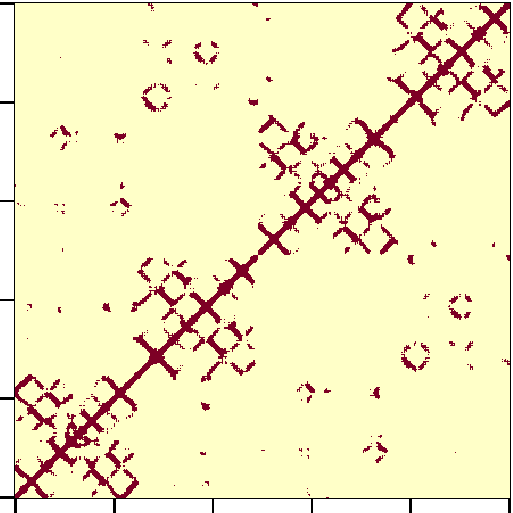
\includegraphics{./stat_dist_files/figure-pdf/fig-contactMatrix-1.pdf}

}

\caption{\label{fig-contactMatrix}Using the \texttt{image} function of
R, we report the contact matrix of the antibody present in the 1nca pdb
file. Each pair of residue are in contact if the distance between their
c-alpha atoms have a distance lower then a certain threshold.}

\end{figure}

In Figure~\ref{fig-contactMatrix} the residue-residue contact matrix for
the antibody of the 1nca pdb is reported.

In order to visualize the number of contacts of each residue, we report
a plot where the residue number and the number of contacts are reported
in the x-axis and y-axis, respectively. Interestingly, by analyzing the
Figure Figure~\ref{fig-contactResidues} is possible to note regions of
the protein with a high number of contacts and regions with low number
of contacts.

\begin{figure}

{\centering 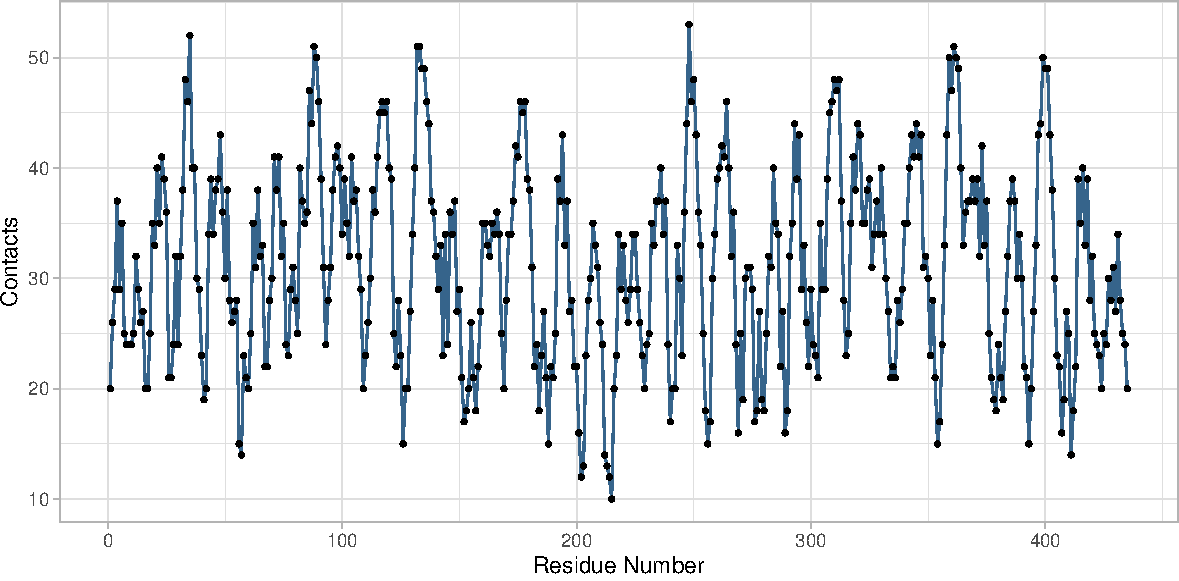
\includegraphics{./stat_dist_files/figure-pdf/fig-contactResidues-1.pdf}

}

\caption{\label{fig-contactResidues}For each residue the number of
contacts is shown. Each pair of residue are in contact if the distance
between their c-alpha atoms have a distance lower then \(12 Å\).}

\end{figure}

In fact, this analysis allow us to analyze some structural properties of
the protein fold: regions with a higher number of contacts are located
in the core of the protein, while regions with fewer contacts are
populated by residues exposed to the solvent.

The purpose of this analysis is to analyze the absolute and relative
frequencies of the number of contacts that each residue has with all its
closest residues.

Therefore, we calculate the number of residues that gave \(n\) contacts,
where \(n\) ranges from 0 to the maximum number of contacts that a
residue can make in this specific protein. We increase the value of
\(n\) by adding 1 contacts to each step of the procedure. In the
following table we report the absolute frequencies, i.e.~how many
residues have 0 contacts, how many residues have 1 contact, how many
residues have 2 contacts, and so on.

\begin{verbatim}
  10 12 13 14 15 16 17 18 19 20 21 22 23 24 25 26 27 28 29 30
1  1  2  2  3  6  4  5  9  6 17 14 14 16 19 18 10 14 16 17 14
\end{verbatim}

\begin{verbatim}
  31 32 33 34 35 36 37 38 39 40 41 42 43 44 45 46 47 48 49 50 51 52 53
1 12 16 16 21 21 11 19 12 17 15 11  4 10  7  4 10  3  4  5  4  4  1  1
\end{verbatim}

For both tables the second row is ``how many residues'' and the first
row is ``have n contacts''. For example, we observe that there 19
residue interacting with 8 residues, as well as, there is 1 residue
interacting with 44 residues.

As described above, we calculate the relative frequency by dividing each
element of absolute frequency by the total number of contacts.

\begin{verbatim}
      10     12     13     14     15     16     17     18     19     20     21
1 0.0023 0.0046 0.0046 0.0069 0.0138 0.0092 0.0115 0.0207 0.0138 0.0391 0.0322
      22     23     24     25
1 0.0322 0.0368 0.0437 0.0414
\end{verbatim}

\begin{verbatim}
     26     27     28     29     30     31     32     33     34     35     36
1 0.023 0.0322 0.0368 0.0391 0.0322 0.0276 0.0368 0.0368 0.0483 0.0483 0.0253
      37     38     39     40
1 0.0437 0.0276 0.0391 0.0345
\end{verbatim}

\begin{verbatim}
      41     42    43     44     45    46     47     48     49     50     51
1 0.0253 0.0092 0.023 0.0161 0.0092 0.023 0.0069 0.0092 0.0115 0.0092 0.0092
      52     53
1 0.0023 0.0023
\end{verbatim}

\bookmarksetup{startatroot}

\hypertarget{references}{%
\chapter*{References}\label{references}}
\addcontentsline{toc}{chapter}{References}

\markboth{References}{References}

\hypertarget{refs}{}
\begin{CSLReferences}{0}{0}
\end{CSLReferences}



\end{document}
